\documentclass[11pt]{article}

\RequirePackage[letterpaper,left=1.0in,top=1.0in,bottom=1.0in,right=1.0in,nohead,nofoot]{geometry}

% Load packages
\usepackage{times}
\usepackage{url}  % Formatting web addresses
\usepackage{ifthen}  % Conditional
\usepackage{multicol}   %Columns
\usepackage[utf8]{inputenc} %unicode support
\usepackage{amsmath}
\usepackage{amssymb}
\usepackage{epsfig}
\usepackage{epstopdf}
\usepackage{graphicx}
\usepackage[font=scriptsize,labelfont=bf]{caption}
\usepackage{setspace}
%\usepackage{longtable}
\usepackage{colortbl}
%\usepackage{palatino,lettrine}
%\usepackage{times}
%\usepackage[applemac]{inputenc} %applemac support if unicode package fails
%\usepackage[latin1]{inputenc} %UNIX support if unicode package fails
\usepackage[wide]{sidecap}
%\usepackage[authoryear,round,comma,sort&compress]{natbib}
%\usepackage[round,sort,comma,numbers,sort&compress]{natbib}
%\usepackage[authoryear,round]{natbib}
\usepackage{supertabular}
\usepackage{simplemargins}
\usepackage{fullpage}
\usepackage{comment}
\usepackage{lineno}
%\usepackage{chicago}
\usepackage{textcomp}
\usepackage{multirow}
\usepackage{amsmath}
\usepackage[linesnumbered,lined,boxed,commentsnumbered]{algorithm2e}
\usepackage{pdflscape} %for rotating pages
\DeclareMathOperator*{\argmin}{\arg\!\min}

\usepackage{algorithm2e}
\usepackage{algpseudocode}
%\usepackage[space]{cite}
\urlstyle{rm}

%\bibliographystyle{chicago}
\usepackage[square,sort,comma,numbers,sort&compress]{natbib}
\usepackage{wrapfig}
\usepackage[font=scriptsize,skip=0pt]{caption}
\makeatletter
\renewcommand\subsection{\@startsection
	{subsection}{2}{0mm}
	{-0.05in}
	{-0.5\baselineskip}
	{\normalfont\normalsize\bfseries}}
\renewcommand\subsubsection{\@startsection
	{subsubsection}{2}{0mm}
	{-0.05in}
	{-0.5\baselineskip}
	{\normalfont\normalsize\bfseries}}
\renewcommand\section{\@startsection
	{subsection}{2}{0mm}
	{-0.2in}
	{0.05\baselineskip}
	{\normalfont\large\bfseries}}
\renewcommand\paragraph{\@startsection
  {paragraph}{2}{0mm}
  {-0.05in}
  {-0.5\baselineskip}
  {\normalfont\normalsize\itshape}}
\makeatother

%Review style settings
%\newenvironment{bmcformat}{\begin{raggedright}\baselineskip20pt\sloppy\setboolean{publ}{false}}{\end{raggedright}\baselineskip20pt\sloppy}

%Publication style settings

% Single space'd bib -
\setlength\bibsep{0pt}

\renewcommand{\rmdefault}{phv}\renewcommand{\sfdefault}{phv}
\newcommand{\norm}[1]{\left\lVert#1\right\rVert}

% Change the number format in the ref list -
\renewcommand{\bibnumfmt}[1]{#1.}

% Change Figure to Fig.
\renewcommand{\figurename}{Fig.}
\everymath{\displaystyle}
\begin{document}
%%%%%%%%%%%%%%%%%%%%%%%%%%%%%%%%%%%%%%%%%%%%%%%%%%%%%%%%%%%%%%%%%%%%%
% TITLE PAGE
%%%%%%%%%%%%%%%%%%%%%%%%%%%%%%%%%%%%%%%%%%%%%%%%%%%%%%%%%%%%%%%%%%%%%
\begin{titlepage}
  \begin{center}
    \vspace*{\stretch{0.8}}
    {\LARGE{Towards a Greater Understanding of Platelet Metabolism}}\par
    \vspace{5em}
    { \Large{Rachel LeCover} \\
    \vspace{1em}
    { \large{ChemE 7700 Final Report}}\par
     \vspace{1em}
    { \large{May 17, 2017}}\par
    \begin{figure}[h]
    \vspace{3em}
       \centering
       
\includegraphics[width=0.7\textwidth]{../figures/CULogo187}
       \end{figure}
    \vspace{2em} \large{ \textit{School of Chemical and Biomolecular Engineering \\ \vspace{0.5em} Cornell University, Ithaca, NY}}}\par
    \vspace{3em}
  \end{center}
\end{titlepage}
\pagebreak

\setcounter{page}{1}
\section*{Background}
Platelets, small anucleate cell fragments produced by megakaryocytes, play a key role in thrombosis, the process of clot formation \cite{hoffman2005hematology}. When the endothelium is damaged and tissue factor(TF) is exposed, the coagulation cascade commences, producing thrombin. Thrombin generation is a positive feed back loop, as thrombin can self activate from its inactive form, prothrombin. Thrombin can bind to the PAR1 receptors, present on the platelet membrane, setting off a signaling cascade inside the platelet that results in the activates PLC$\beta$ (phospholipase C$\beta$), which catalyzes the conversion of PIP$_2$ (phosphatidylinositol 4,5-bisphosphate) to IP$_3$(inositol 1,4,5 trisphosphate) and DAG \cite{brass2003thrombin}. The increased IP$_3$ leads to a release of calcium from the platelet's dense tubular system, which leads to an influx of calcium into the platelet from the surrounding fluid. The spike in intracellular calcium increases the activity of PLA2 (phospholipase A2), which catalyzes the production of TXA$_2$ (thomboxane A2). Activated platelets then dump the contents of their dense granules (vesicles containing ADP) into the surroundings. This ADP then interacts with the P2Y1 receptor, resulting in the inhibition of adenlyate cyclcase, and a decrease in cAMP concentration, allowing for a change in platelet shape \cite{hoffman2005hematology}. Additionally, the presence of this additional calcium results in the movement of phosphatidlyserine (PS) to the outer layer of platelet membranes \cite{lhermusier2011platelet}.

The prothombinase complex, consisting of active factors X and V, forms on the surfaces of platelets during coagulation\footnote{If you are unfamiliar with the coagulation cascade, TF activates FVII, and forms the TF-FVIIa complex, which activates FIX and FX. FX can catalyze the production of thrombin from prothrombin, but not very quickly. However, once a small amount of thrombin is generated, this thrombin can activate FV, FVIII, and FXI. The [FV-FX]$_a$ complex is very good at activating thrombin, and the [FIX-FVIII]$_a$ complex activates additional FX, resulting in a positive feed back loop.}. This complex is very efficient at activating thombin-the complete complex (with phosophlipids, FXa, FVa, and calcium)\footnote{The a denotes active} has a $V_{max}$ of 1919 mol/min per mol FXa, compared to a $V_{max}$ of .61 mol/min per mol FXa in the presence of only FXa \cite{rosing1980role}. Phophoditylserine is key to the formation of the prothominase complex and to the normal function of the coagulation cascade, and if the scrablease that moves phophtidylserine to the outer leaflet of the membrane does not function properly, the patient will suffer from a bleeding disorder, known as Scott syndrome \cite{halliez2015detection}. 

\subsection*{Previous Work}
Since platelets play a key role in homeostasis, we may wish to understand platelet metabolism and activation. A fairly comprehensive kinetic model of platelet signaling exists, containing 77 reactions and 70 species \cite{purvis2008molecular}, however, this model does not include the activation of platelets by thrombin. In 2014, Thomas et al published a model of platelet metabolism based on evidence from 33 human platelet proteomic studies \cite{thomas2014network}. This model contains 1008 reactions (mapped to 636 genes) and 739 compartment specific metabolites, but lacks any sort of a control system or signal transduction mechanism.  

\section*{Extension of Literature}
I extended the platelet metabolic model developed by Thomas et al by adding logical rules to simulate platelet activation and by transforming it into a dynamic model as opposed to a static one. To mimic signaling, I changed the bounds of the model in response to the external concentrations of activating molecules (calcium, TXA$_2$, and ADP). By extending this model, I hoped to understand how platelet metabolism changes during activation, and if a model that had been built to describe metabolism at steady state would change when a perturbation was applied. 
\section*{Mathematical Methods}
\subsection*{Flux Balance Analysis (FBA)}
FBA permits the solving of undertermined systems of equations, such as those found describing the flow of metabolites through a cell. This technique was used by Thomas et al to solve their model of platelet metabolism. Instead of seeking a solution for the underdetermined system of equations (Equation \ref{stoch}), it recasts the problem as a maximization problem, as shown in Equation \ref{max}, which can be solved via linear programming techniques, such as the Simplex method.
\begin{equation}
\max_{v_1,...v_R}\sum_{i=1}^Rc_iv_i
\label{max}
\end{equation}
Subject to:
\begin{equation}
Sv=b
\label{stoch}
\end{equation}

\begin{equation}
L_i  \leq \sum_{i=1}^R \sigma_{ij}v_j \leq U_i
\end{equation}

\begin{equation}
\alpha_j \leq v_j \leq \beta_j
\end{equation}
In the above equations, $v_i$ represents a flux through the system, $c_i$ is the weight applied to the flux in the objective, $S$ is the stoichiometric matrix (with elements $\sigma_{ij}$), $b$ is the residual (usually set to zero), $L_i$ is the lower species bound for species $i$, $U_i$ is the upper, $\alpha_j$ is the lower bound for flux $j$, $\beta_j$ is the upper bound on it.
\subsection*{Dynamic Flux Balance Analysis (dFBA)}
Dynamic flux balance analysis extends flux balance analysis to examine changes in flux as external conditions change, as reflected in changes in the bounds applied to the system, as shown in Equations \ref{speciesbounds} and \ref{fluxbounds}.  
\begin{equation}
\max_{v_1,...v_R}\sum_{i=1}^Rc_iv_i
\end{equation}
Subject to:
\begin{equation}
Sv=\frac{dy}{dt}
\end{equation}
\begin{equation}
\label{speciesbounds}
L_i(t)  \leq \sum_{i=1}^R \sigma_{ij}v_j(t) \leq U_i(t)
\end{equation}

\begin{equation}
\label{fluxbounds}
\alpha_j(t) \leq v_j(t) \leq \beta_j(t)
\end{equation}
The main change is that the product of the stoichiometric matrix and the flux vector is no longer a constant, rather, it represents the changes in the concentrations of the species in the system $\frac{dy}{dt}$. This differential equation is solved by first solving the linear programming problem for $v$, and then integrating the results at discrete time points through Euler's method. I used dFBA to make the platelet model respond to changes in the external environment. Normally, for FBA or dFBA problems, an objective is chosen that maximizes cell growth or the production of a protein of interest. Since my platelets were not growing nor producing any proteins, I instead maximized the production of energetic species-ADP, NADH, and NADPH, as previously done in a model of a red blood cell \cite{tekir2006analysis}.
\section*{Results}
\subsection*{Inducing activation with ADP}
By changing the bounds with respect to external ADP and calcium concentrations, I was able to mimic the deterministic simulation in \cite{purvis2008molecular}, as shown in Figure \ref{fig:ADPspike}. 
\begin{wrapfigure}[21]{l}{.55\textwidth}
\vspace{-.5cm}
\centering
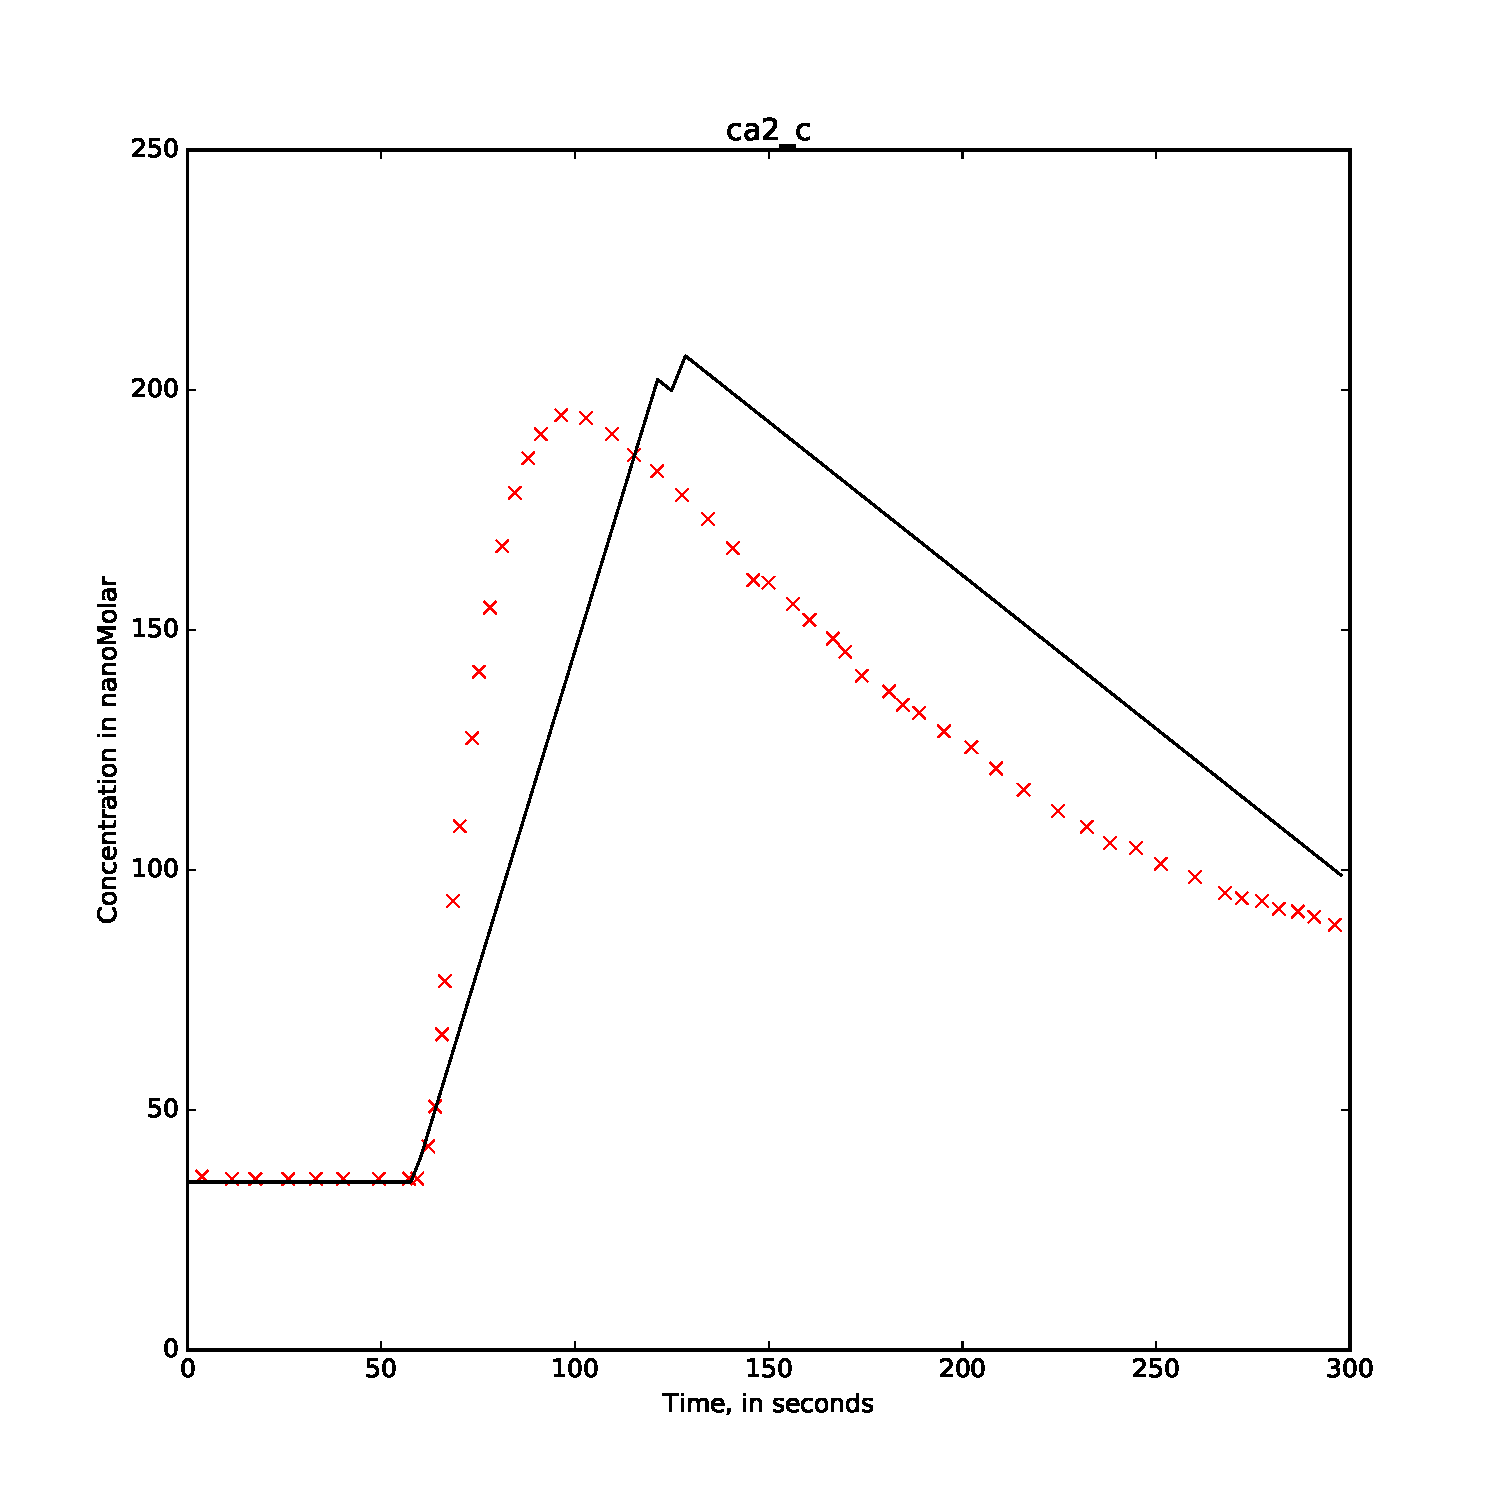
\includegraphics[scale=.35]{../figures/internalCa}
\caption{Red X are data from \cite{purvis2008molecular}, black line is the dFBA simulation. This figure was generated by increasing the external ADP concentration to 20 $\mu$M at 60 seconds.}
\label{fig:ADPspike}
\end{wrapfigure}
Although far from a perfect fit, by changing the bounds I was able to capture the increase in internal calcium concentration up to about 200 $\mu$M and its subsequent decline. In order to capture this behavior, I allowed calcium to accumulate in the model's cytoplasmic compartment, which is generally not permitted in FBA. If we compare the the flux distributions between steady state and activation, we can see that there are significant changes in platelet metabolism, especially in glycolylsis, as shown in Figure \ref{fig:Ca_glycolysis}, and in exchange reactions, shown in the supplemental material (Figure S\ref{fig:Ca_Exchange}). Some fluxes remain the same in both cases, such as the flux through aldehyde dehydrogenase (ADD2Y) and glyceraldehyde-3-phosphate dehydrogenase (GAPD), but others are quite different. PGMT (phosphoglucomutase, the conversion of g1p(glucose 1 phosphate) to g6p (glucose 6 phosphate)) turns on, as does the flux through triose-phosphate isomerase, which produces glucose 6 phosphate from dihydroxyacetone phosphate. The flux through ENO also increases, resulting in increased production of phosphoenolpyruvate from glycerate 2-phosphate when the platelet is activated. Although the model predicts changes in the fluxes through glycolysis, experiments with radioactively labeled carbon would need to be carried out to validate these predictions. 
\begin{figure}
\centering
\hspace{-2cm}
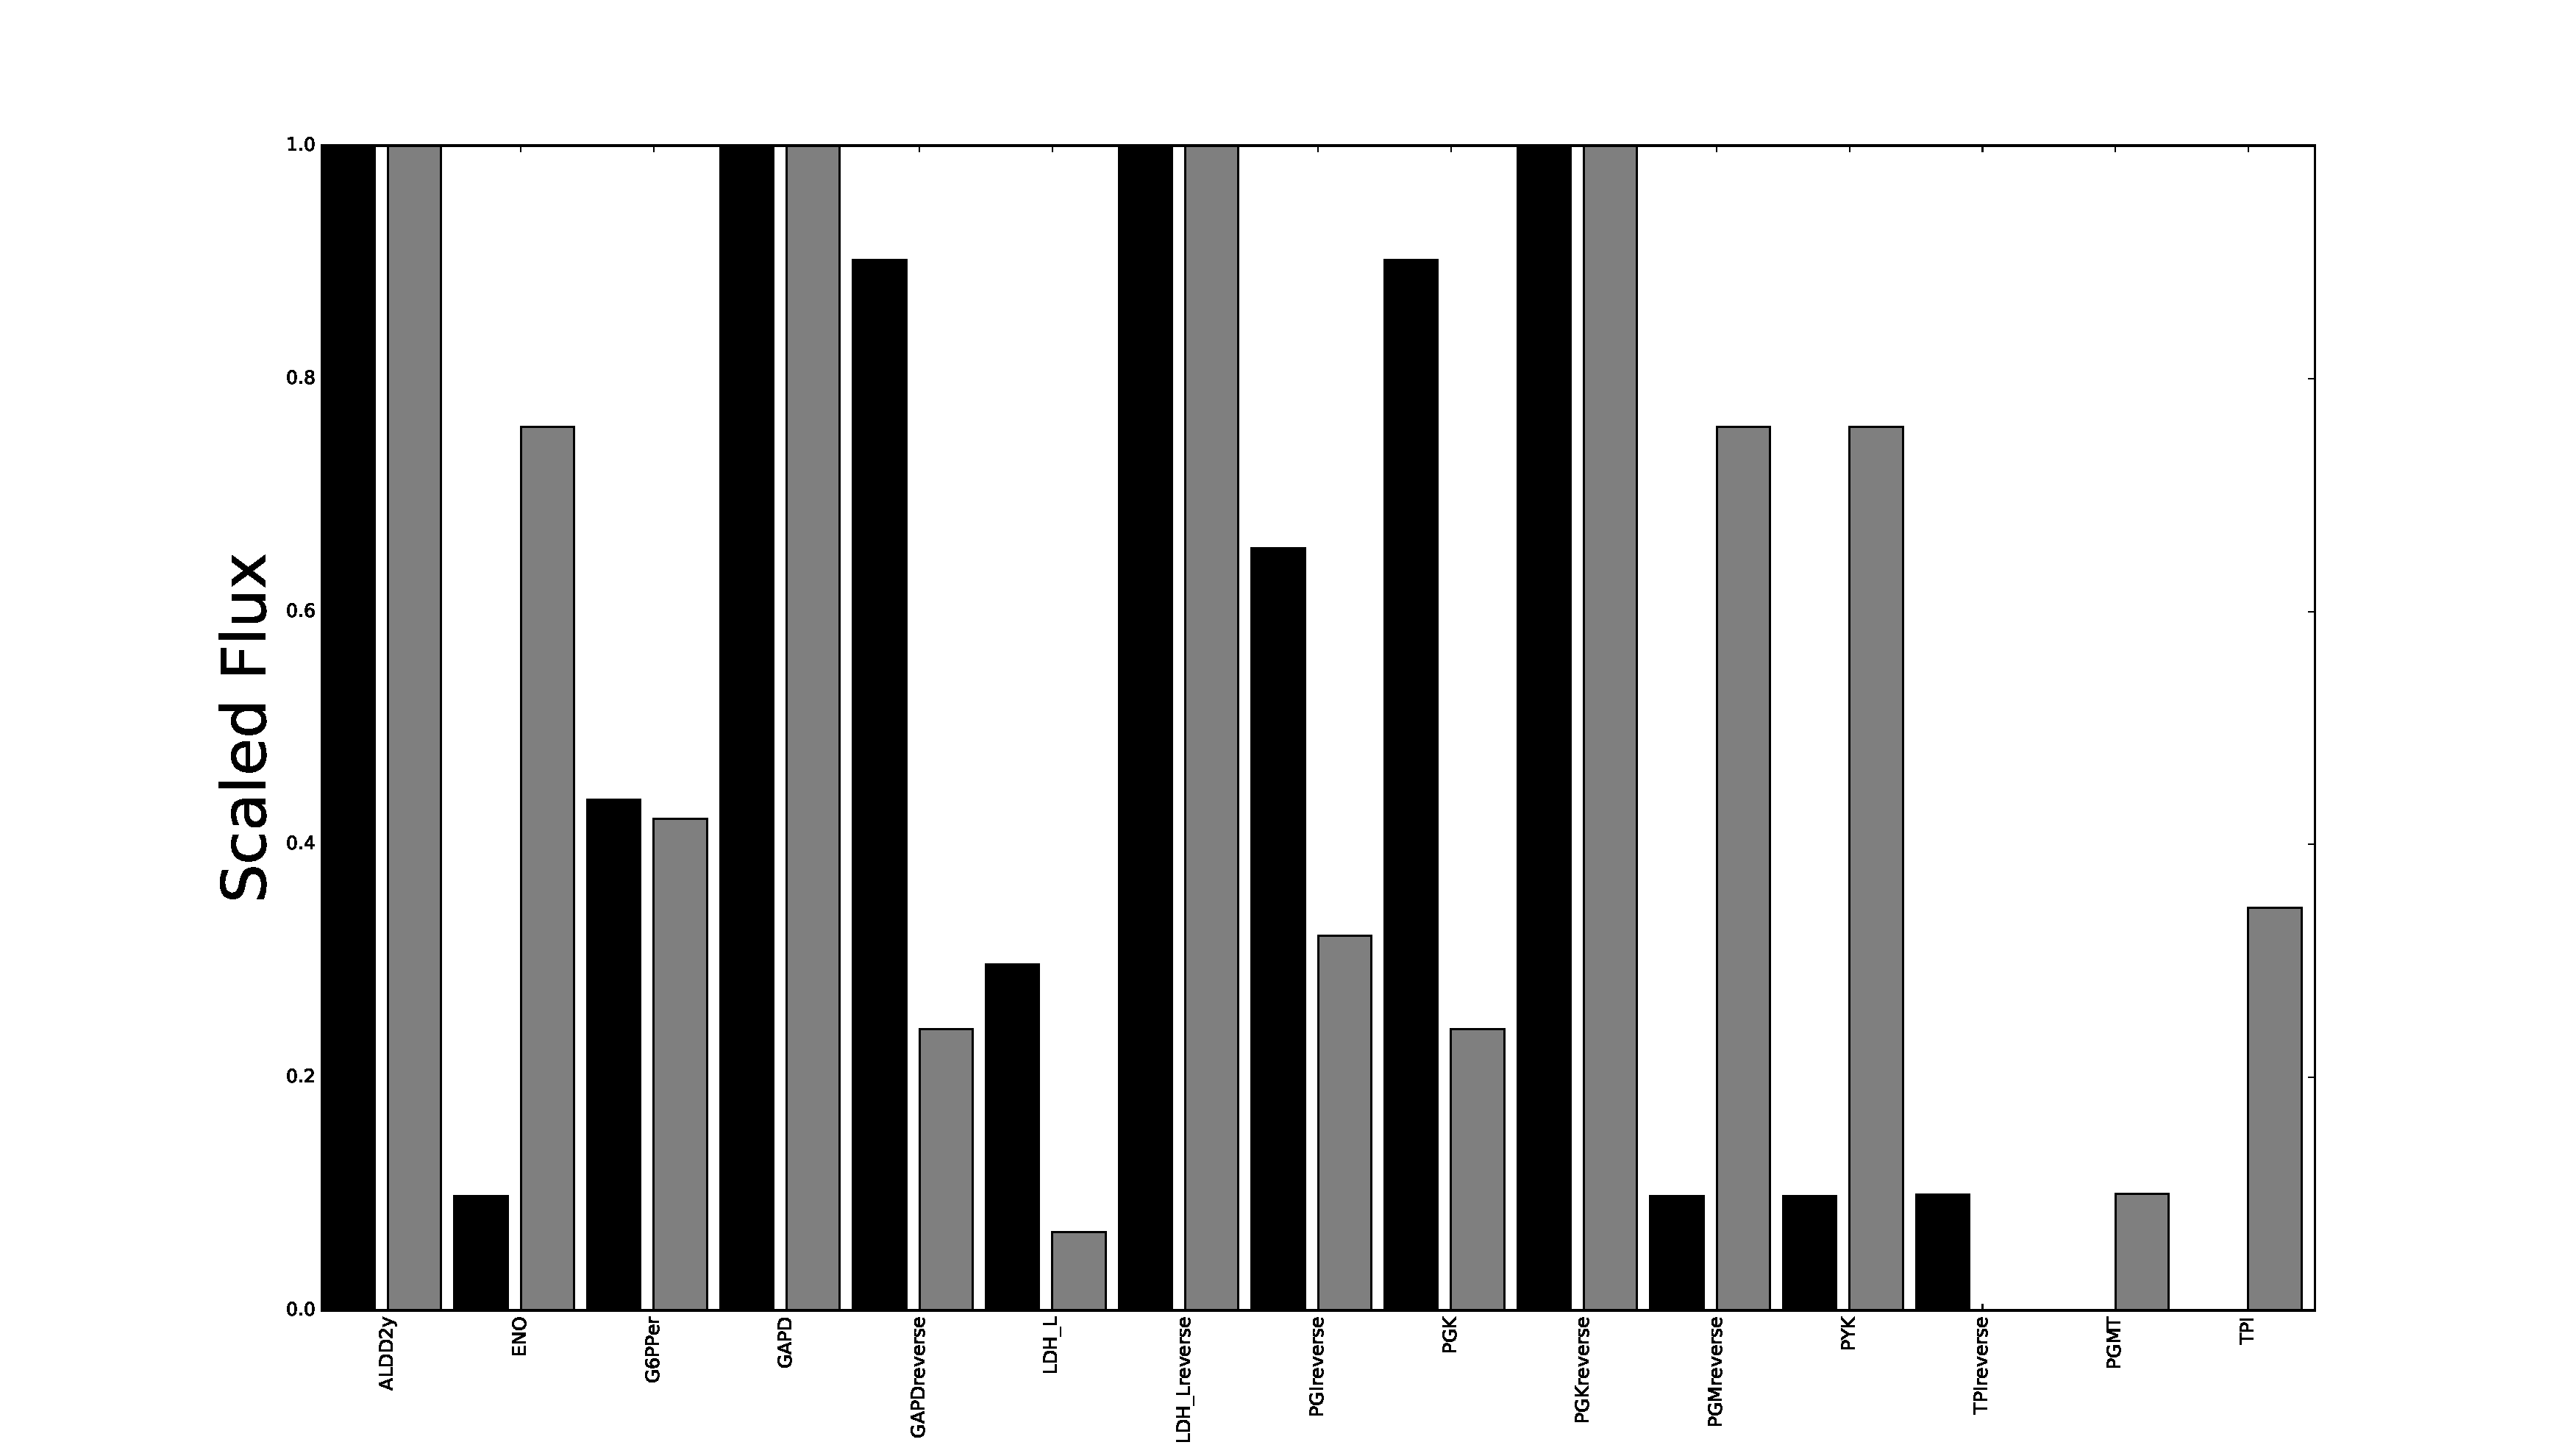
\includegraphics[scale=.25]{../figures/Ca_barGlycolysis_Gluconeogenesis}
\caption{Comparison of fluxes through glycolysis and gluconeogensis at steady state (black) and during the platelet activation process (gray). Fluxes are scaled by dividing by the upper limit on fluxes.}
\label{fig:Ca_glycolysis}
\end{figure}
\subsection*{Gene Knock Outs}
\begin{wrapfigure}[17]{l}{.55\textwidth}
\vspace{-.5cm}
\centering
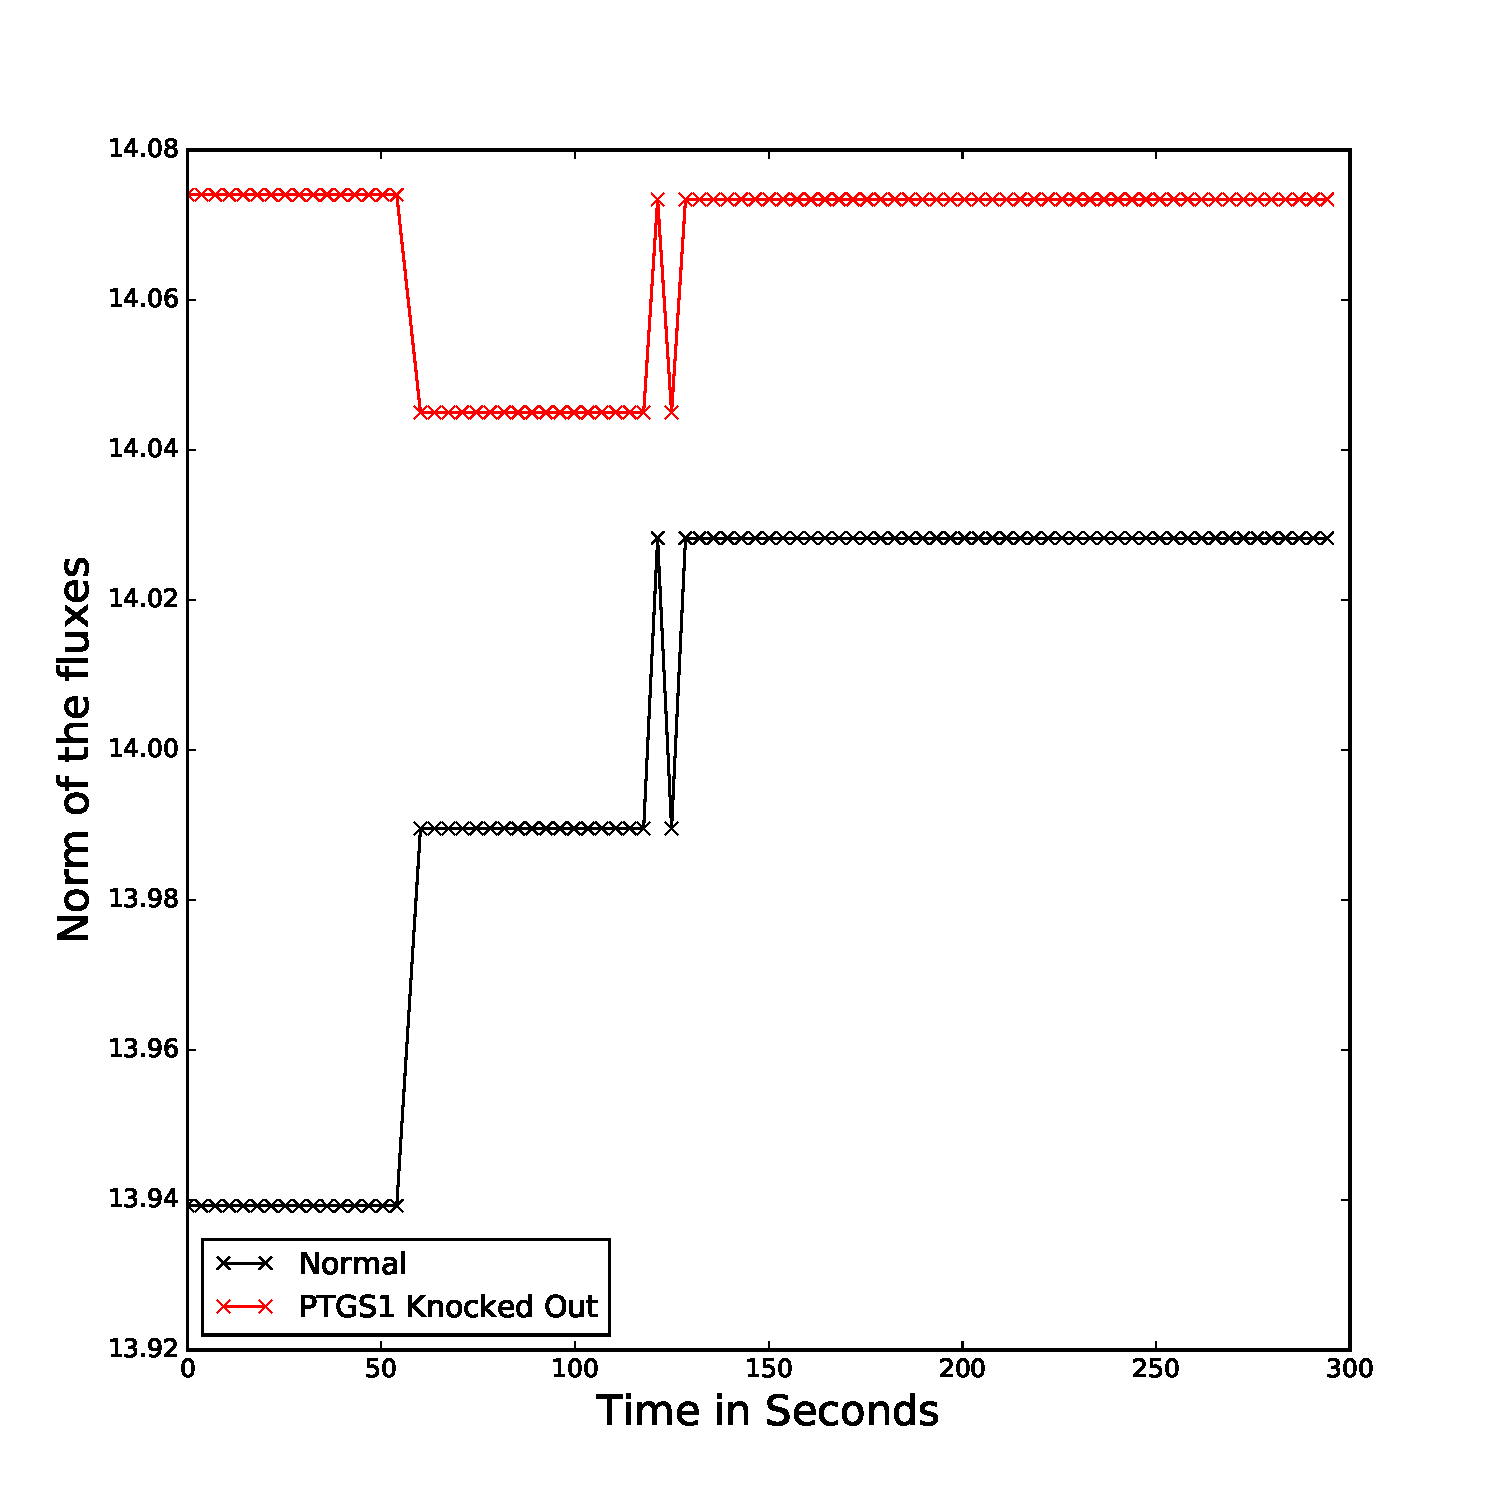
\includegraphics[scale=.35]{../figures/NormOfFluxesNormalAndKnockedCaSpike}
\caption{Differences between the norms of the fluxes between wild type and platelet with flux through reactions dependent on PTGS-1 forcibly reduced.}
\label{fig:normfluxes}
\end{wrapfigure}
As previously described, the model of platelet metabolism which I extended links many of its fluxes to genes, including PTGS-1, prostglandin-enoperoxide synthase 1 (also known as cylclooxygenase-1 (COX-1)). PTGS-1 codes for the enzyme that converts arachidonic acid to prostgladin, which is later converted into TXA$_2$, a key molecule in platelet signaling and activation \cite{kunicki2010genetics}. I wished to examine how platelet metabolism would alter if the flux through these reactions was significantly decreased, simulating a mutation that negatively effected the efficiency of COX-1. (A complete knock out resulted in a linear programming problem that was not primal feasible, so I instead lowered the upper bound on these fluxes to one tenth of the nominal upper bound). Even at steady state, before activation, there were significant differences between the wild type and altered platelet, as shown in Figure \ref{fig:SSknockout}. When the flux through PTGS-1 is forcibly reduced, the flux through fructose-bisphophate aldolase (FBA) and through phosphofrutokinase (PFK) falls to nearly zero. To quantify the changes between the normal and knockout platelet throughout the activation process, I examined the norm of the fluxes, plotted in Figure \ref{fig:normfluxes}, which clearly shows that there are significant differences between the flux distribution in all phases: steady state, activation (increasing cytosolic calcium) and deactivation (decreasing cytosolic calcium). Examining the differences between the steady state exchange fluxes between the knock out and wild type lead to an interesting realization-many of the fluxes that turn on in the knock out that weren't on in the wild type have sodium participate in their reactions (Figure S\ref{fig:knockoutExchangeSS}).
\begin{wrapfigure}[16]{l}{.55\textwidth}
\vspace{-.5cm}
\centering
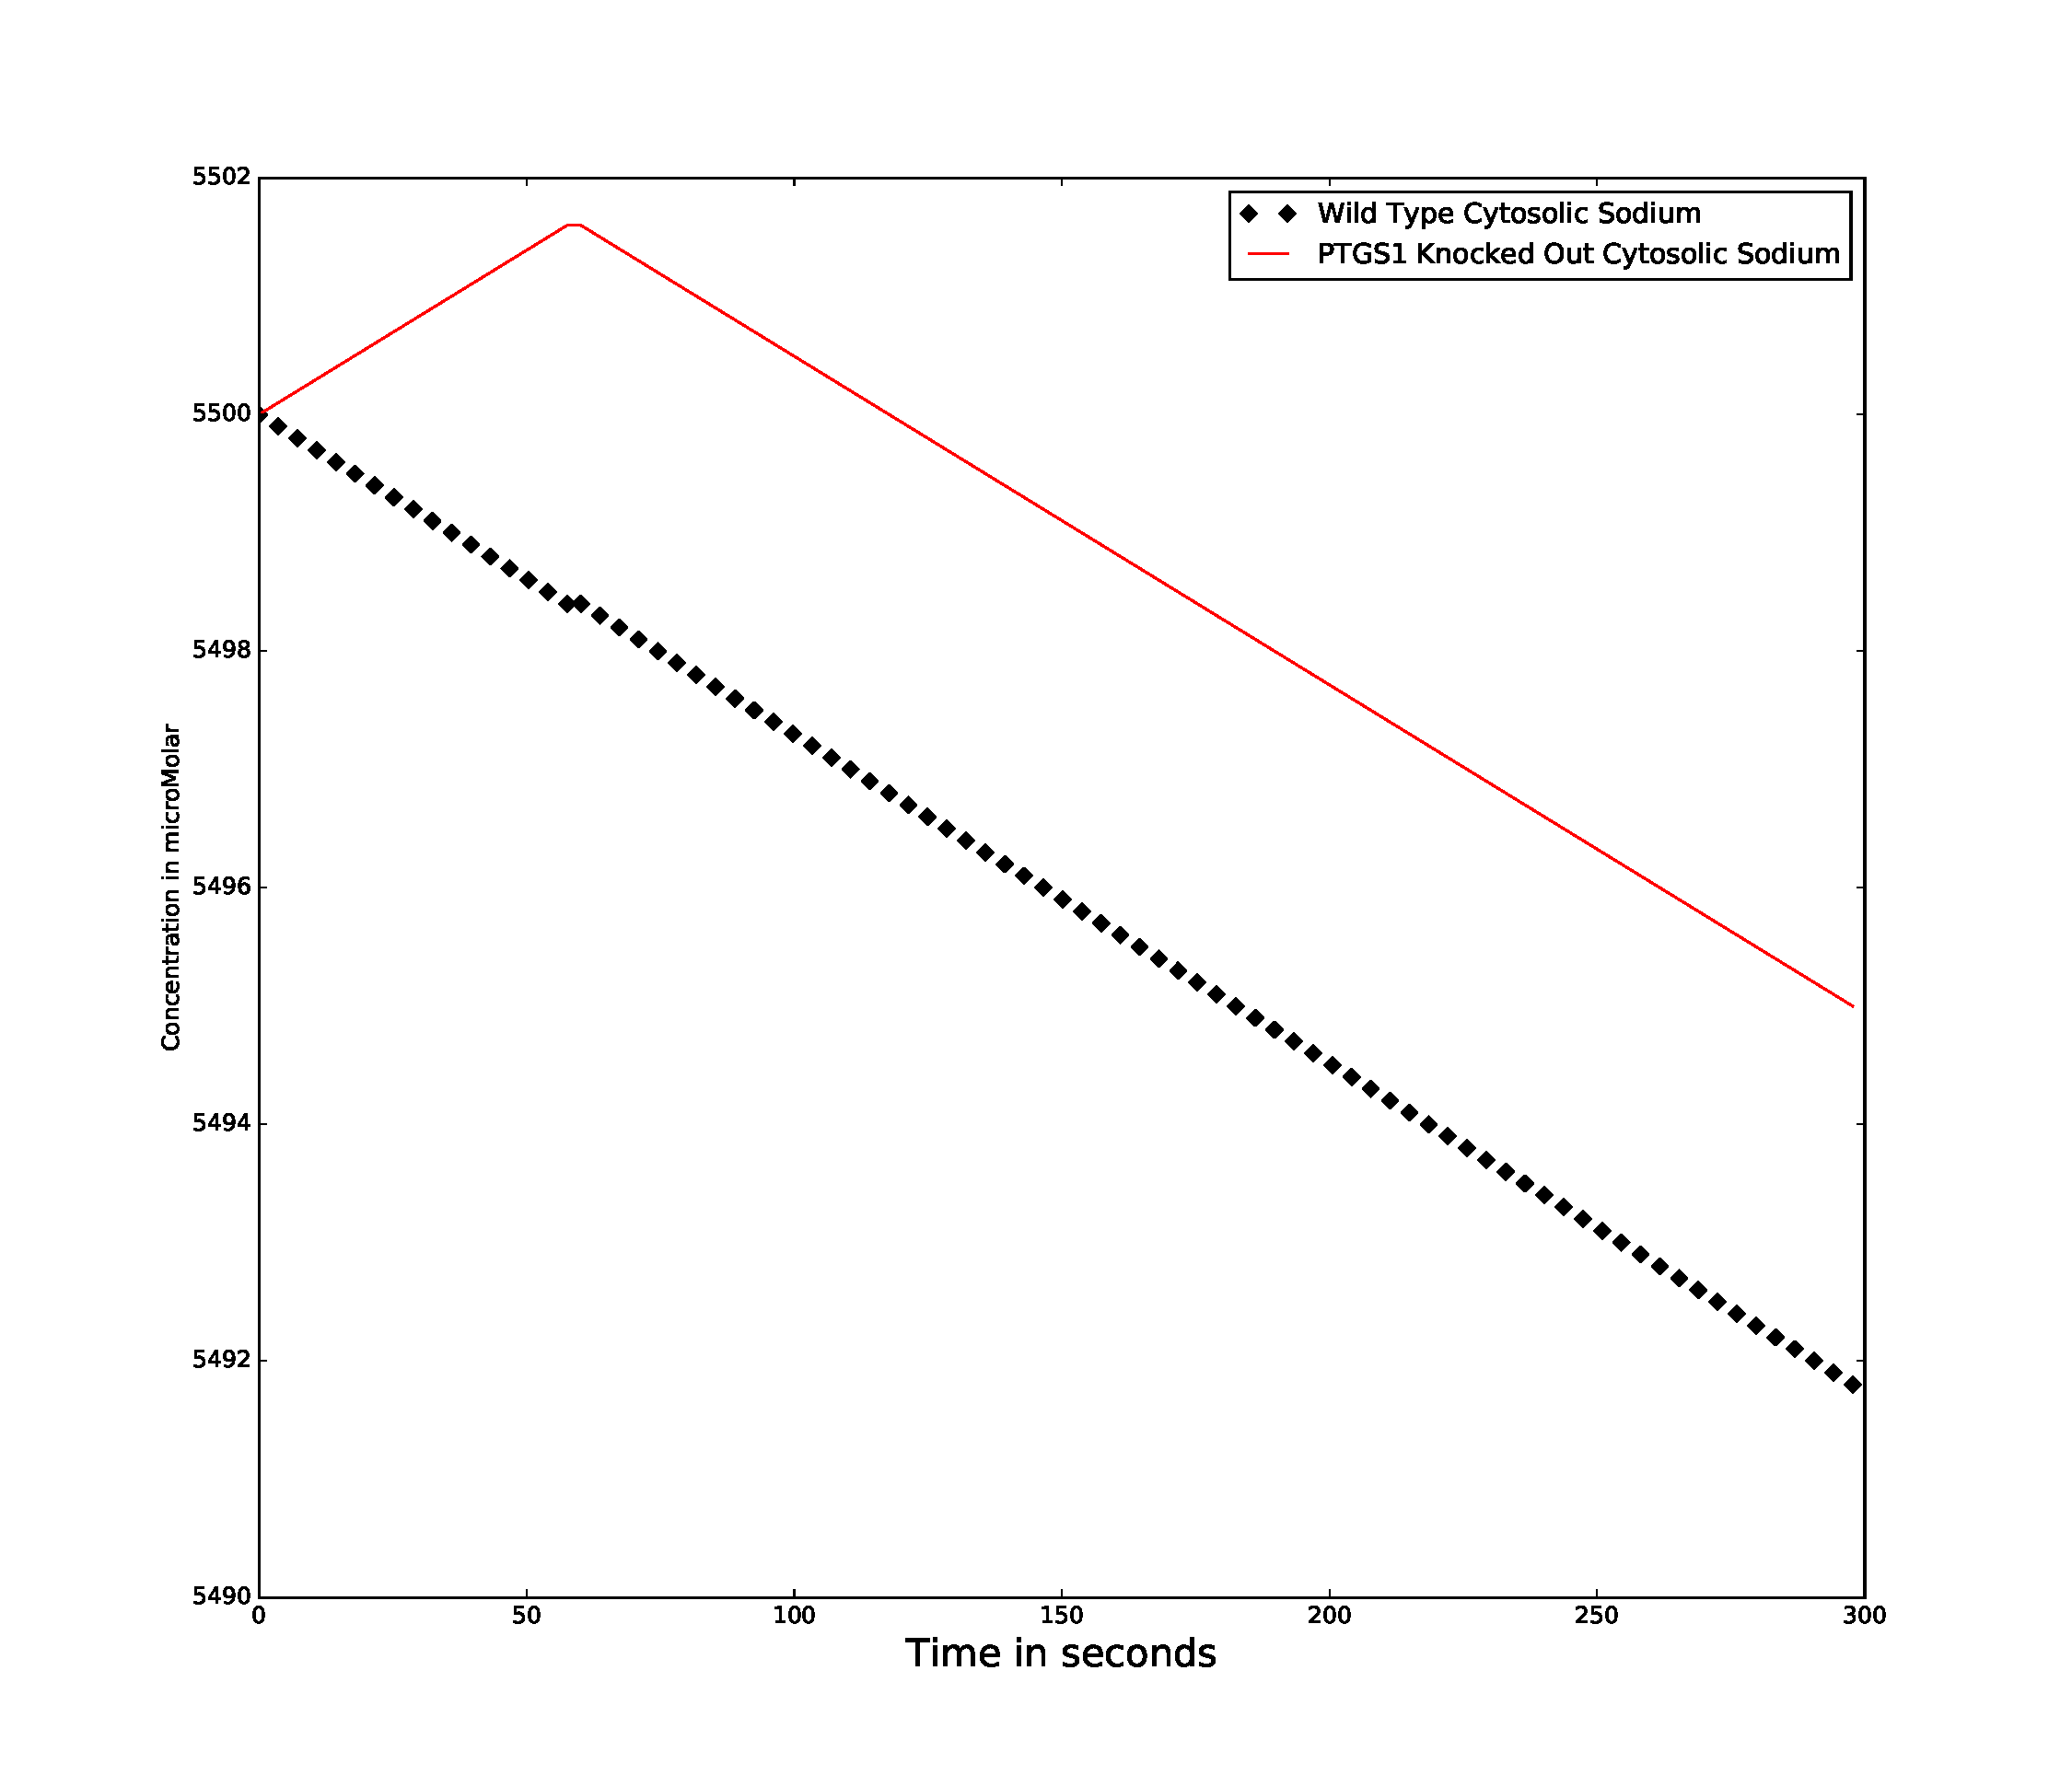
\includegraphics[scale=.25]{../figures/cytosolicNa}
\caption{Differences between the cytosolic concentration of sodium in platelets with and without a fully functional PTGS-1 gene. Sodium was permitted to accumulate in both cases. Cytosolic sodium initial condition is taken from  \cite{sage1991resting}. }
\label{fig:cytoNa}
\end{wrapfigure}

\begin{figure}
\centering
\hspace{-2cm}
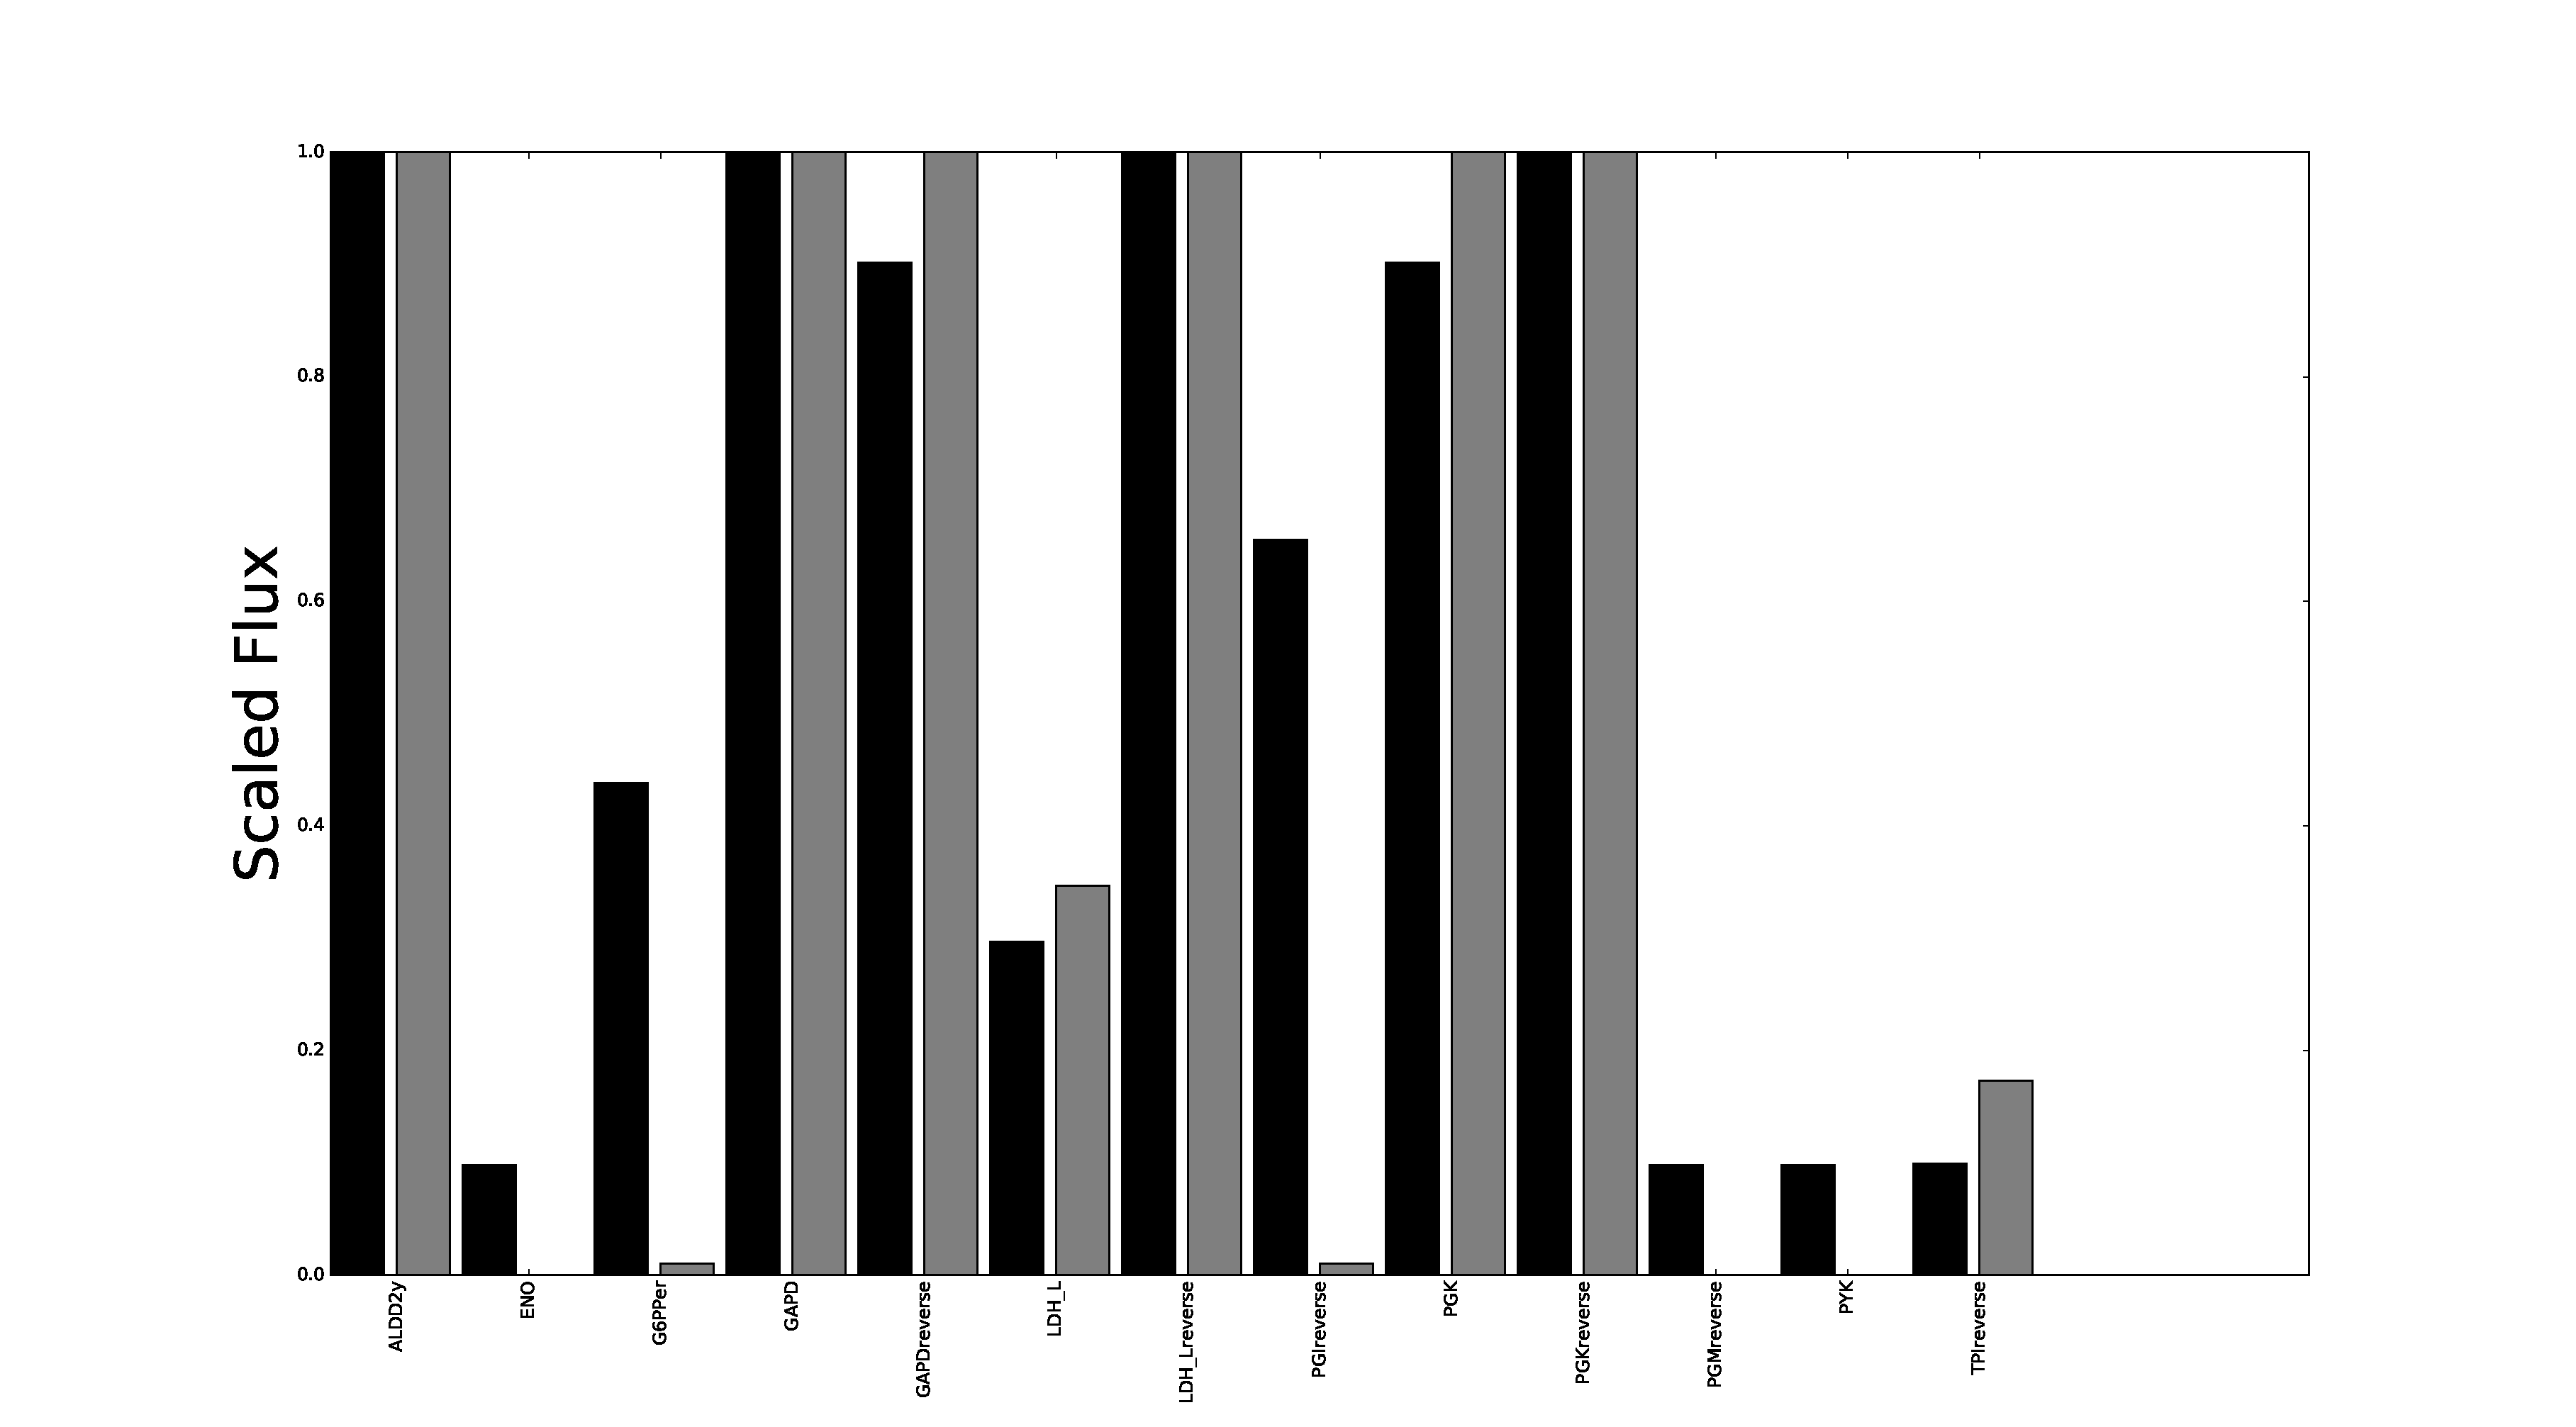
\includegraphics[scale=.25]{../figures/barSSKnockouts[5742,5743]Glycolysis_Gluconeogenesis}
\caption{Comparison of fluxes through glycolysis and gluconeogensis at steady state for wild type (black) and knockout platelet (gray). Fluxes are scaled by dividing by the upper limit on fluxes.}
\label{fig:SSknockout}
\end{figure}
This led me to alter the model to allow sodium to accumulate in the cytosol, and compare the sodium profiles between the wild type and knock out platelets, as shown in Figure \ref{fig:cytoNa}, in which there is a clear difference between the two types of platelets. This discovery led me to search the literature, and I discovered that platelets are known to import sodium when stimulated with ADP, a behavior that I had not created a logical rule to simulate \cite{sage1991resting}. As a result, my wild type simulated platelets exported sodium throughout the simulation, and when stimulated, the knockout platelets had the opposite behavior as expected-they exported sodium instead of uptaking it. Father review of the literature lead me to believe that sodium also plays a role in platelet activation-when the cytosolic concentration of sodium is increased the $K_d$ (dissociation constant) for epinephrine increases, so that it is more likely to disassociate from the receptors on the platelet surface \cite{motulsky1983influence}. \footnote{Epinephrine is a known inducer of platelet aggregation \cite{spalding1998mechanism}}

\section*{Conclusions}
I was successful in constructing a dFBA model of platelet metabolism from a previously existing FBA model, and in implementing a system to knock out or reduce the fluxes that had attached gene regulation. Furthermore, I was able to mimic a portion of the signaling cascade involved in platelet activation and observe that there are significant changes in platelet metabolism during the activation process, even though this model lacked many of the key responses to activation (granule secretion and cytoskeletal rearrangement). However, this model has many shortcomings, as evidenced by the sodium profile that goes counter to experimental evidence. For a better understanding of platelet metabolic changes during activation, a more comprehensive regulatory layer would need to be added that better captures all the known signaling cascades. KEGG contains a reference platelet signaling map which would provide a starting point for construction of this regulatory layer \cite{kanehisa2017kegg}, however, the existing FBA model would have be significantly altered to include key regulatory proteins before this comprehensive model could be constructed.
\section*{Acknowledgments}
Many thanks to Mike Vilkhovoy for providing assistance in setting the correct conditions for my FBA problem so that it would solve.

\bibliographystyle{unsrt}
\bibliography{report}

\section*{Supplemental Material}
\setcounter{figure}{0}    %restart figure numbering
\renewcommand{\figurename}{S}
\begin{landscape}
\begin{figure}
\hspace{-2cm}
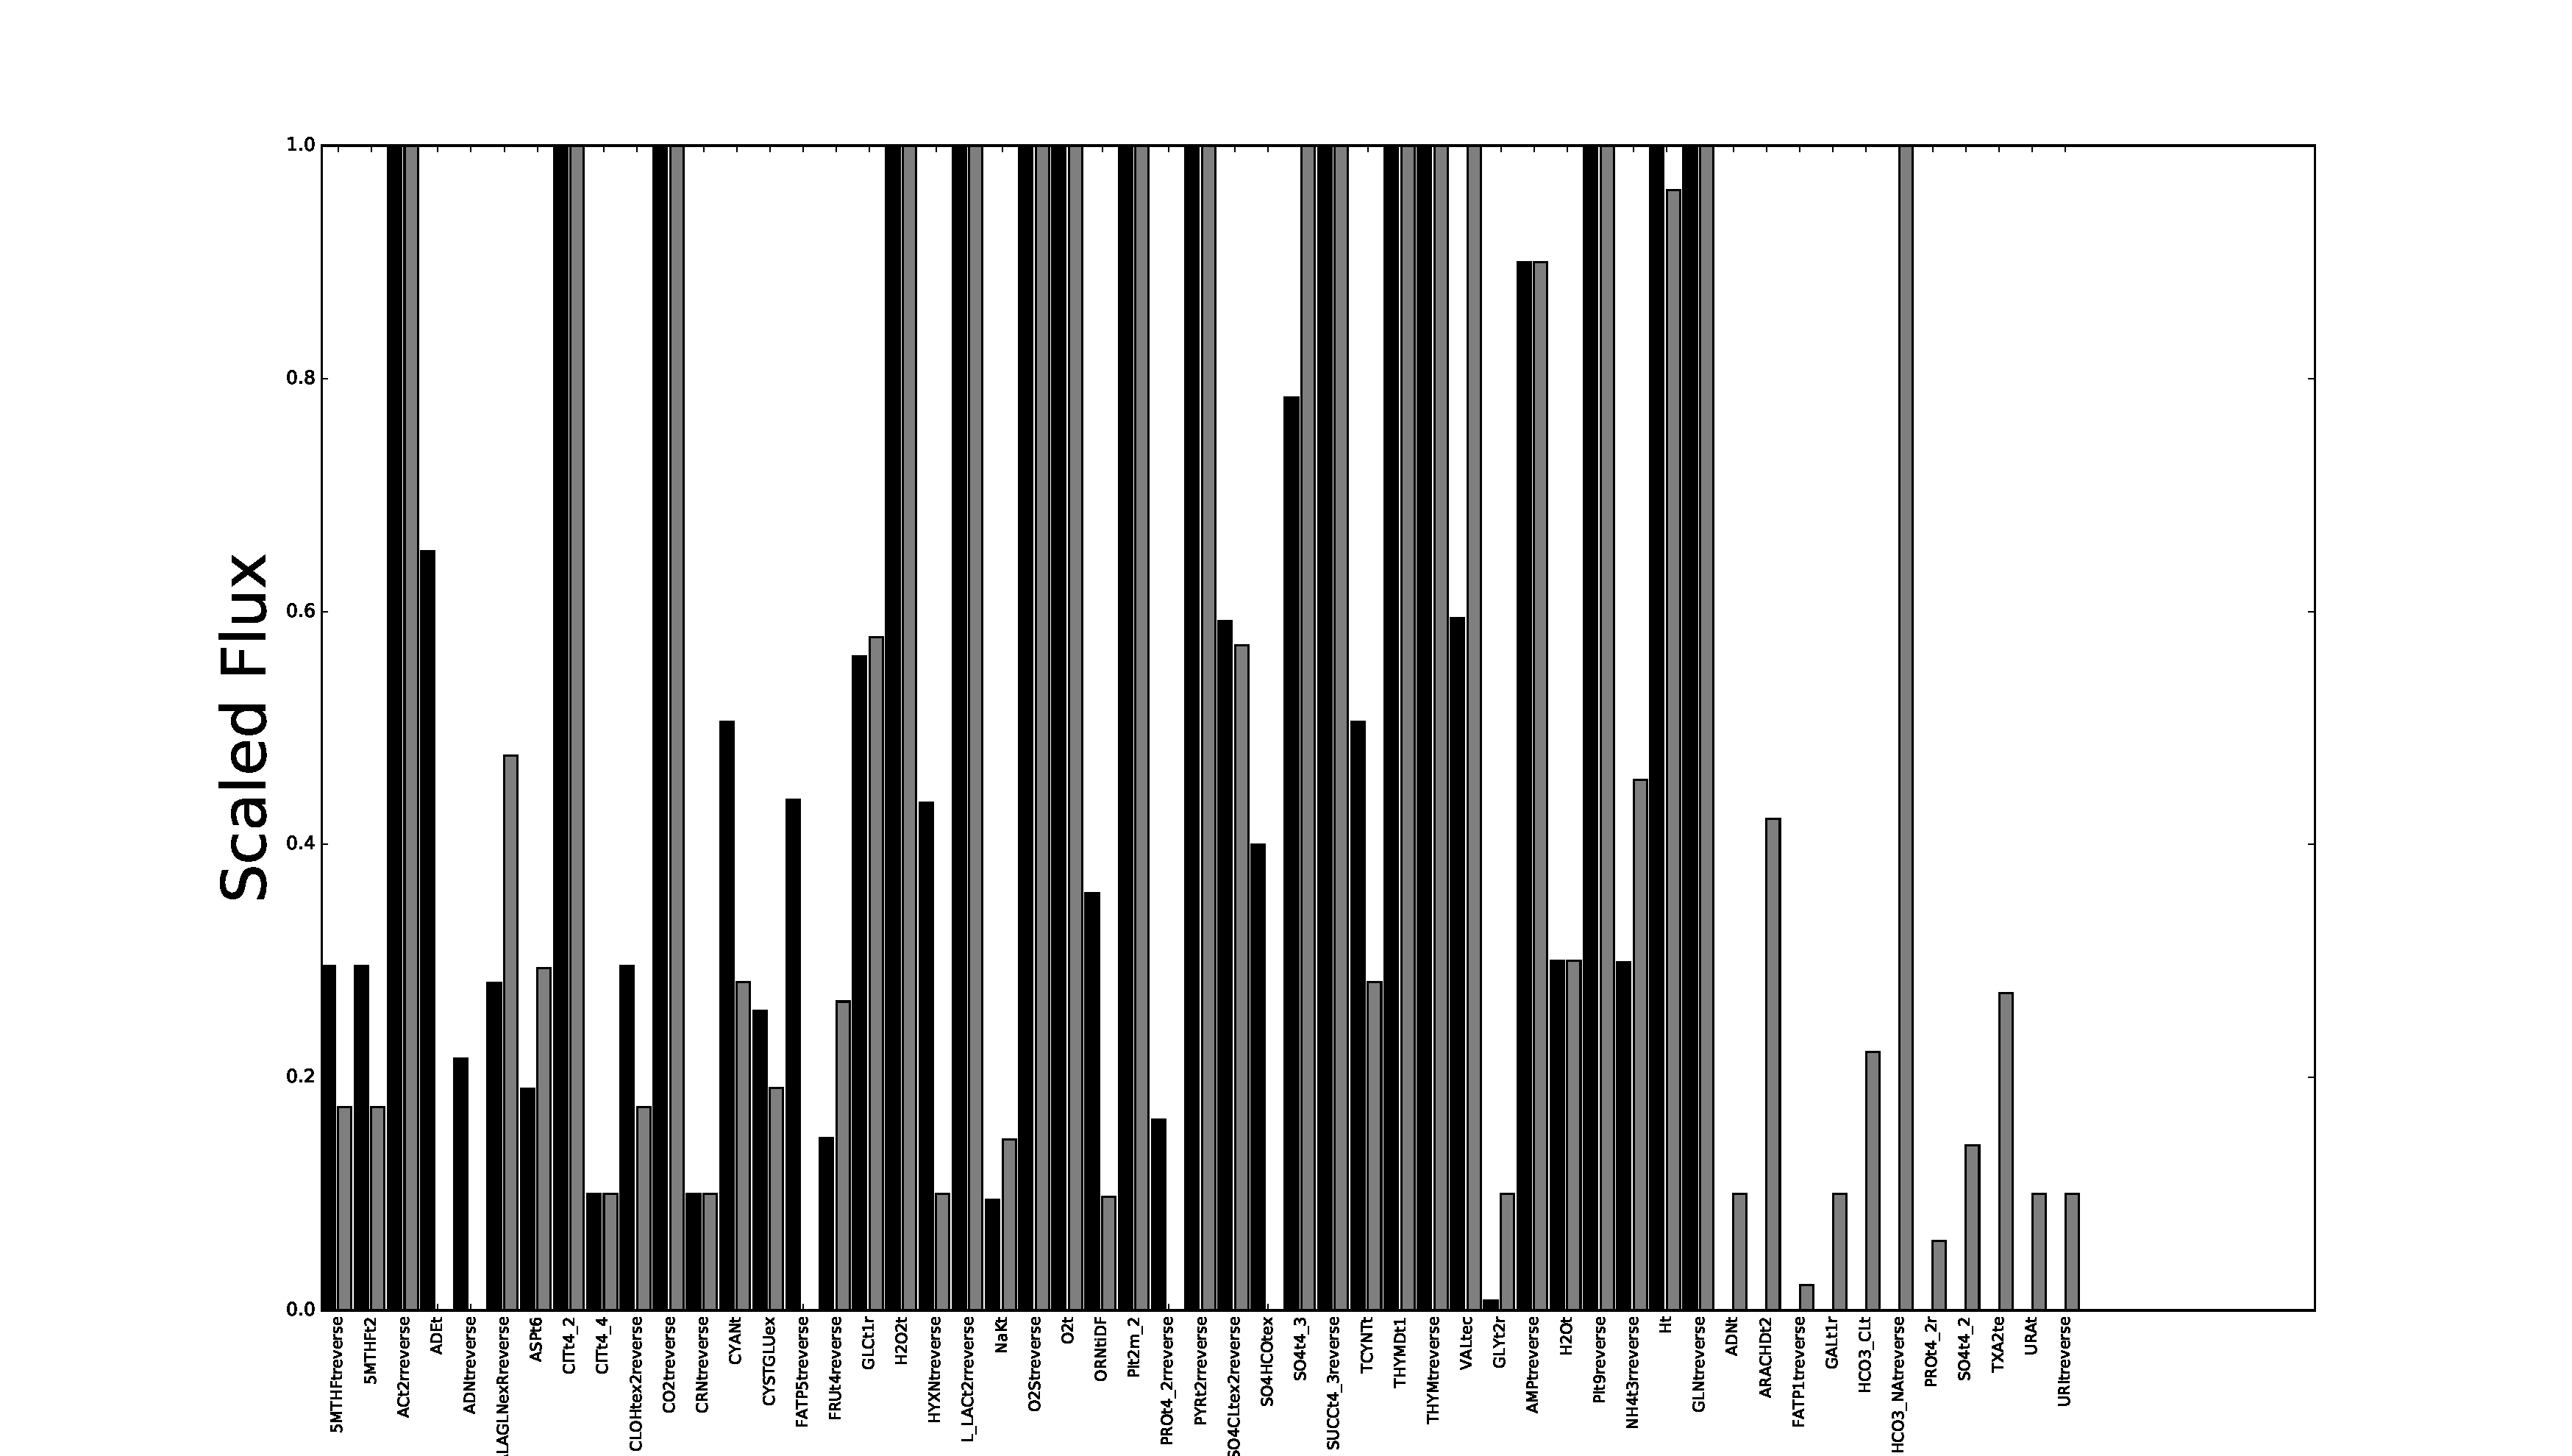
\includegraphics[scale=.55]{../figures/Ca_barTransport_Extracellular}
\caption{Comparison of exchange fluxes at steady state (black) and during the platelet activation process (gray). Fluxes are scaled by dividing by the upper limit on fluxes.}
\label{fig:Ca_Exchange}
\end{figure}

\begin{figure}
\hspace{-2cm}
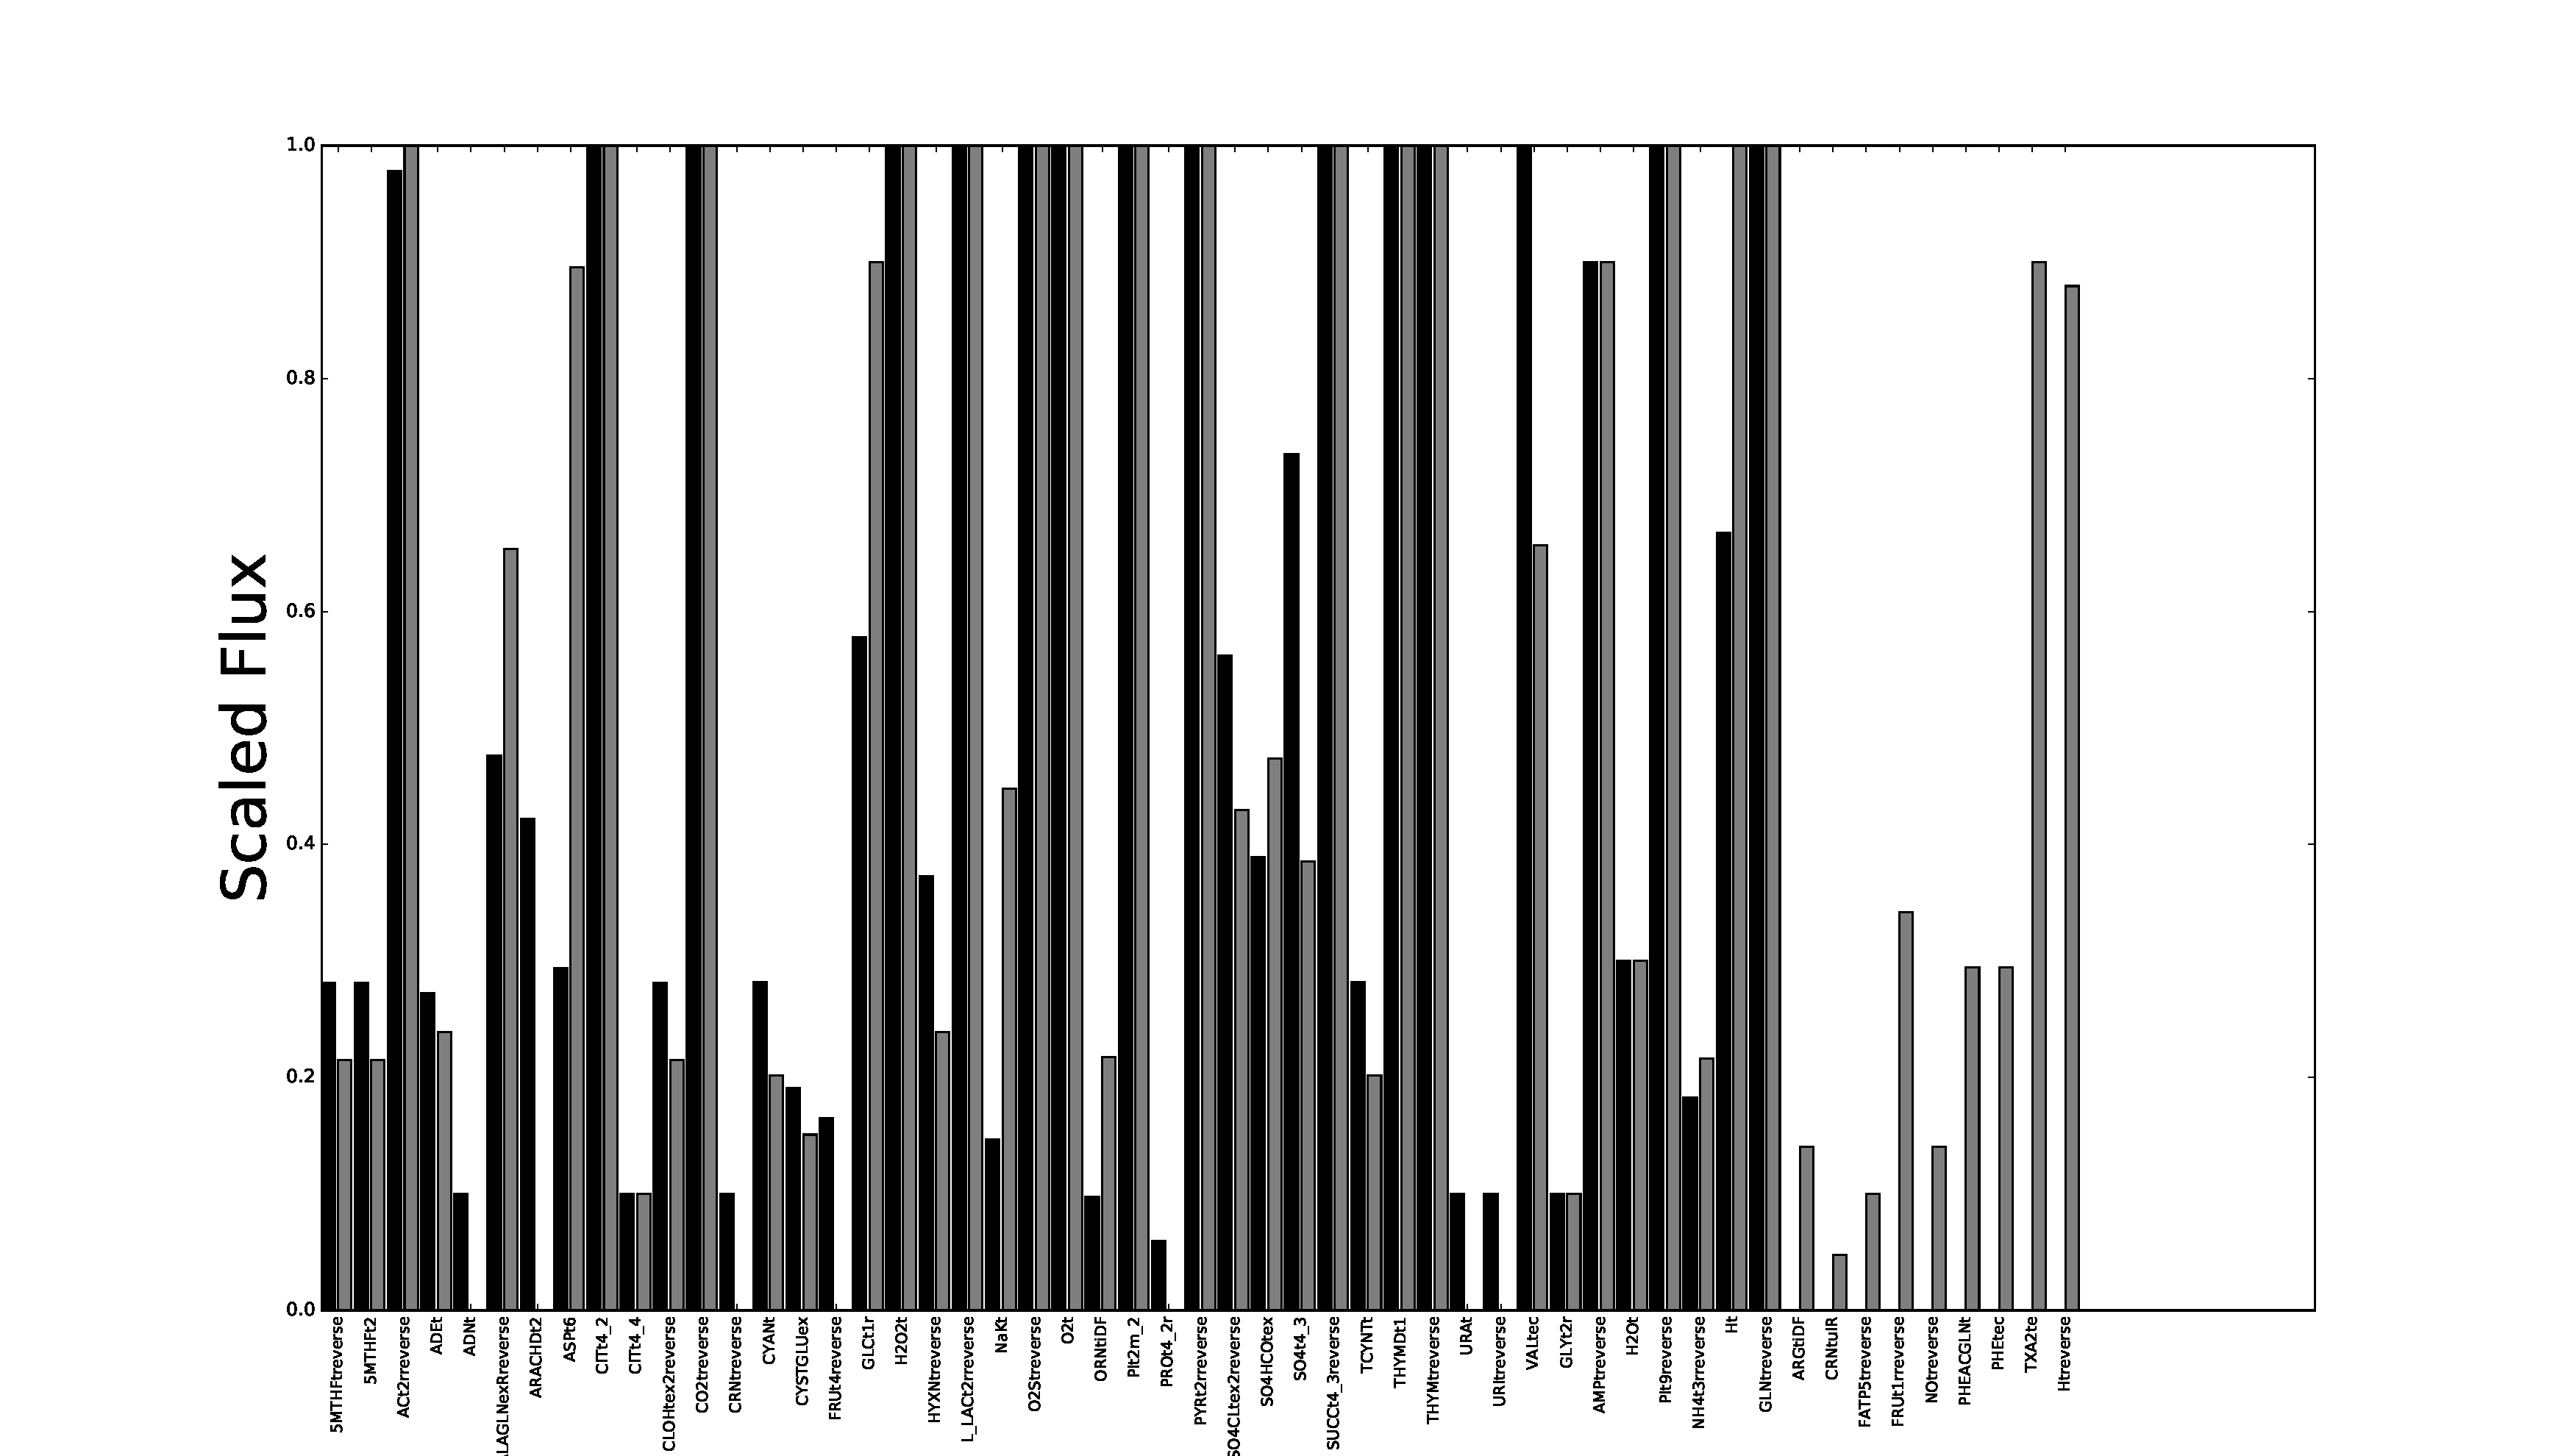
\includegraphics[scale=.55]{../figures/barSSKnockouts[5742,5743]Transport_Extracellular}
\caption{Comparison of exchange fluxes at steady state for wild type (black) and knockout platelet (gray). Fluxes are scaled by dividing by the upper limit on fluxes.}
\label{fig:knockoutExchangeSS}
\end{figure}
\end{landscape}
\end{document}
